\documentclass{endm}
\usepackage{endmmacro}
\usepackage{graphicx}
\usepackage{amsmath}

% The following is enclosed to allow easy detection of differences in
% ascii coding.
% Upper-case    A B C D E F G H I J K L M N O P Q R S T U V W X Y Z
% Lower-case    a b c d e f g h i j k l m n o p q r s t u v w x y z
% Digits        0 1 2 3 4 5 6 7 8 9
% Exclamation   !           Double quote "          Hash (number) #
% Dollar        $           Percent      %          Ampersand     &
% Acute accent  '           Left paren   (          Right paren   )
% Asterisk      *           Plus         +          Comma         ,
% Minus         -           Point        .          Solidus       /
% Colon         :           Semicolon    ;          Less than     <
% Equals        =           Greater than >          Question mark ?
% At            @           Left bracket [          Backslash     \
% Right bracket ]           Circumflex   ^          Underscore    _
% Grave accent  `           Left brace   {          Vertical bar  |
% Right brace   }           Tilde        ~

\newcommand{\Nat}{{\mathbb N}}
\newcommand{\Real}{{\mathbb R}}
\def\lastname{Brito}

\begin{document}  

% DO NOT REMOVE: Creates space for Elsevier logo, ScienceDirect logo
% and ENDM logo
\begin{verbatim}\end{verbatim}\vspace{2.5cm}

\begin{frontmatter}

\title{On the Fast Creation of Conflict Graphs for Integer Programs: A Computational Study}

\author{Samuel Souza Brito\thanksref{myemail} \and Haroldo Gambini Santos\thanksref{coemail}}
 
\address{Computing Department\\ Universidade Federal de Ouro Preto - UFOP\\ Ouro Preto, Brazil}
\thanks[myemail]{Email:
   \href{mailto:samuelsouza@iceb.ufop.br} {\texttt{\normalshape
   samuelsouza@iceb.ufop.br}}} \thanks[coemail]{Email:
   \href{mailto:haroldo@iceb.ufop.br} {\texttt{\normalshape
   haroldo@iceb.ufop.br}}}

\begin{abstract}
Conflict graphs are employed in modern Integer Programming to store relationships between variables. This information is crucial for an effective pre-processing and cut generation. CGs can be dynamically built inside branch-and-bound algorithms while analyzing the impact of the last fixations performed, but the earlier the CG is populated the faster strong inequalities and implications can be generated. On this work we present techniques which allow the fast creation of densely populated CGs at the root node. The impact of the availability of these large GCs for cut generation is evaluated by the inclusion of these techniques in the state-of-the-art open source integer programming solver COIN-OR CBC and its use in a cutting plane algorithm.
\end{abstract}

\begin{keyword}
conflict graphs, integer programming, clique cuts, set packing polytope
\end{keyword}

\end{frontmatter}


\section{Introduction}\label{intro}

In this work we present an approach for the creation of conflict graphs for Integer Programming (IP) problems. A Conflict Graph (CG) represents logical relations between binary variables. This kind of graph has a vertex for each binary variable and its complement. An edge between two vertices indicates that variables involved cannot be set to some specific value at the same time without violating one or more constraints.

CGs are typically constructed using probing techniques \cite{Borndorfer1998} based on constraints analysis. The probing technique consists in analyzing logical implications generated by fixing binary variables. For example, in a given problem the activation of the variable $x$ implies the deactivation (i.e. activation of its complement) of the variable $y$, in order to respect the constraints of the problem. In this case, we found a an implication in the form $x = 1 \ \Rightarrow \ y = 0$, which would add the edge $(x,y)$ to the graph.

Building a graph by looking for pairwise of conflicts may be computationally prohibitive when the input problem is large. Thus, the computational efficiency of this technique depends on the complexity of the constraint exploration, causing a trade off between efficiency and effectivity. 

One important application for CGs is the generation of cutting planes derived from the Set Packing Polytope\cite{Padberg1973}, such as the Clique Inequalities. The dynamic inclusion of these inequalities allows tightening the linear relaxation of an IP problem, improving performance of branch-and-bound based solvers \cite{atamturk}. Hoffman and Padberg \cite{hoffman} used conflict graphs to generate valid inequalities for set partitioning problems arising in airline crew-scheduling. Achterberg \cite{achterberg} presented heuristics based on SAT techniques for Mixed Integer Programming solvers to generate valid inequalities from the current infeasible subproblem and the associated branching information. The same idea has been developed independently and in parallel by Sandholm and Shields \cite{sandholm}.  

On this work we propose techniques to speed up the creation of dense conflict graphs at the root node, so that large CGs can be available at the start of the search process for the generation of strong inequalities. For ease of understanding of our approach we consider only pure Binary Programs (PB). Despite this, it can be applied to any Integer Program containing binary variables. 

The rest of the paper is organized as follows. In Section \ref{seccgraph}, we formally explain our approach to build conflict graphs as well our strategy to speedup the detection of logical implications. In Section \ref{cut}, we present the clique cut separation routine, including a clique extension step. In Section \ref{experiments}, the computational experiments with MIPLIB 2010 instances \cite{miplib} and instances of the International Nurse Rostering Competition \cite{haspeslagh} are presented and analyzed. Finally, in Section \ref{conclusions}, we conclude and give future directions about this work.

\section{Conflict Graphs in Integer Programming}\label{seccgraph}

A conflict graph represents logical relations between binary variables. For two binary variables, we may discover four possible logical relations, using the notation of \cite{atamturk}:

\begin{align}
x = 1 \Rightarrow y = 1 & \quad \Longleftrightarrow \quad x + (1 - y) & \leq \ 1\\
x = 1 \Rightarrow y = 0 & \quad \Longleftrightarrow \quad x + y & \leq \ 1 \\
x = 0 \Rightarrow y = 1 & \quad \Longleftrightarrow \quad (1 - x) + (1 - y) & \leq \ 1 \\
x = 0 \Rightarrow y = 0 & \quad \Longleftrightarrow \quad (1 - x) + y & \leq \ 1
\end{align}

Given an Integer Programming (IP), a conflict graph can be constructed using probing techniques based on feasibility considerations. The basic idea is to analyze the impact of activation or deactivation (i.e. activation of its complement) of two variables at time, for each pair of variables and each constraint. Each constraint $i \in \{1,\ldots,m\}$ can be written as:

\begin{equation}
 \sum_{j \in N} a_{ij}x_{j} \leq b_{i} 
\end{equation}

\noindent where $N$ is the index set of binary variables $x$, $a_{ij}$ is the coefficient for variable $x_{j}$ at constraint $i$ and $b_{i}$ is the right-hand side of constraint $i$. Suppose we are analyzing two particular variables $x_{\hat{j}}$ and $x_{\hat{k}}$ with respect to constraint $i$. Consider that these variables are assigned with values $u$ and $v$, respectively. Let:

\begin{equation}\label{li}
L_{i}^{x_{\hat{j}} = u,\, x_{\hat{k}} = v}=\sum_{j\in N_{i}^{-} \setminus \{\hat{j}, \hat{k}\}}a_{ij}+a_{i\hat{j}}u+a_{i\hat{k}}v 
\end{equation}

\noindent where $N_{i}^{-} = \{j \in N : a_{ij} < 0\}$. In this case, $L_{i}^{x_{\hat{j}} = u,\, x_{\hat{k}} = v}$ is a lower bound for the value on the left-hand side  of the constraint $i$, considering the assignments $x_{\hat{j}} = u$ and $x_{\hat{k}} = v$. If $L_{i}^{x_{\hat{j}} = u,\, x_{\hat{k}} = v} > b_{i}$, there is a conflict between the assignments of $x_{\hat{j}}$ and $x_{\hat{k}}$. 

Performing these steps for each combination of values of two binary variables, considering each pair of variables in each constraint, leads to the creation of a conflict graph for any IP problem in $O(m \times n^2)$. For problems with many variables and constraints this technique may be too expensive computationally (See Experiments section). Nevertheless, for some constraint types a large number of conflicts can be quickly discovered. This is the case of the Generalized Upper Bound constraints ($\sum_{j\in N}x_j \leq 1$). As discussed in \cite{atamturk}, even handling explicitly conflict graphs induced by these constraints requires special data structures such that in the previous decade most solvers could not use all information which could be inferred just from GUB constraints. The following subsection will describe additional cases where cliques in constraints can be quickly detected (i.e., faster than $O(n^2)$). The following notation will be used: $\tilde{a}_{ik}$ is the $k$-th smallest coefficient in constraint $i$ and $\acute{a}_{ik}$ indicates its index. Constants $n_i$ and $S_i^-$ denote the number of non-zero variables and the sum of all negative coefficients of constraint $i$, respectively. To illustrate one case, GUB constraints can be described as $\tilde{a}_{ik}=b_i=1 \ \forall \ k$. In the next subsection fast clique detection will be discussed for additional constraint structures.


\subsection{Fast detection of cliques in less structured constraints}

We describe two simple cases where large cliques of conflicting variables can be detected just by traversing constraints with  coefficients of variables sorted in non-decreasing order. Thus, conflicts in these constraints are discovered in $O( n \log n)$.

To detect cliques that involve the activation of some variables we start computing the lower bound of the left-hand side (LHS) for each two consecutive variables, starting the analysis from the smallest coefficient ($k=1$) to the highest one ($k=n_i$). The first step is compute the sum of negative coefficients excluding the two analyzed variables:

\begin{equation}\label{di}
D_{i}^{x_{\acute{a}_{ik}}, x_{\acute{a}_{ik+1}}} = S_i^- - min(0, \tilde{a}_{ik}) - min(0, \tilde{a}_{ik+1})
\end{equation}

\noindent Thus, the lower bound for the LHS of constraint $i$ when variables with $k$ and $k+1$ smallest coefficients are fixed at one is:

\begin{equation}
LHS_{i}^{x_{\acute{a}_{ik}} = 1, x_{\acute{a}_{ik+1}} = 1} = D_{i}^{x_{\acute{a}_{ik}}, x_{\acute{a}_{ik+1}}} + \tilde{a}_{ik} + \tilde{a}_{ik+1}
\end{equation}

Since $LHS_{i}^{x_{\acute{a}_{ik}} = 1, x_{\acute{a}_{ik+1}} = 1}$ is monotonically non-decreasing as $k$ increases, if $LHS_{i}^{x_{\acute{a}_{ik}} = 1, x_{\acute{a}_{ik+1}} = 1} > b_{i}$, then there is a clique involving the activation of all variables from position $k$ until position $n_i$. Moreover, we can discard the existence of such cliques by checking if $LHS_{i}^{x_{\acute{a}_{in_i-1}} = 1, x_{\acute{a}_{in_i}} = 1} \leq b_i$.

The same idea can be used to detect cliques that involve the deactivation of some variables, computing the lower bound of the LHS for each two consecutive variables, starting from the highest coefficient ($k=n_i$) to the smallest one ($k=1$). The lower bound for the LHS of constraint $i$ when variables $x_{\acute{a}_{ik}}$ and $x_{\acute{a}_{ik-1}}$ are fixed at zero is equal to $D_{i}^{x_{\acute{a}_{ik}}, x_{\acute{a}_{ik-1}}}$, which is obtained by equation \ref{di}:  $LHS_{i}^{x_{\acute{a}_{ik}} = 0, x_{\acute{a}_{ik-1}} = 0} = D_{i}^{x_{\acute{a}_{ik}}, x_{\acute{a}_{ik-1}}} $


In the same form, $LHS_{i}^{x_{\acute{a}_{ik}} = 0, x_{\acute{a}_{ik-1}} = 0}$ is monotonically non-decreasing as $k$ decreases. If $LHS_{i}^{x_{\acute{a}_{ik}} = 0, x_{\acute{a}_{ik-1}} = 0} > b_{i}$, then there is a clique involving the deactivation of all variables from position $k$ until the variable of first position ($k=1$). Moreover, we can discard the existence of such cliques by checking if $LHS_{i}^{x_{\acute{a}_{i2}} = 0, x_{\acute{a}_{i1}} = 0} \leq b_i$.

When no clique is found we use the pairwise analysis. Nevertheless, in our experiments we observe a large number of constraints that have cliques, speeding up the creation of conflict graphs.

\begin{example}

Consider the following constraints as a part of an IP problem, where all variables are binary:

\begin{align}
x_1 + x_2 + x_3  & \geq 2\label{eq:1}\\
- 2x_1 + 3x_2 + 4x_3 + 5x_4 & \leq 4\label{eq:2}
\end{align}

\begin{figure}[!ht]
  \begin{center}
    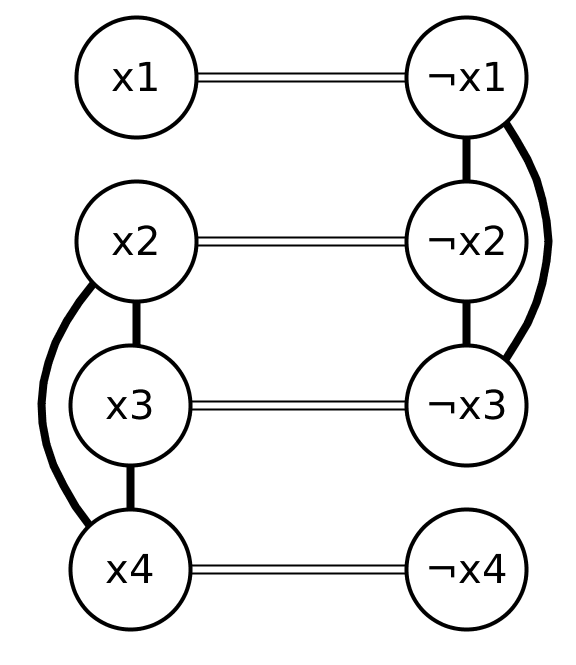
\includegraphics[width=4cm]{graph.png}
  \end{center}
  \caption{A conflict graph for constraints presented in equations \ref{eq:1} and \ref{eq:2}.}
  \label{graph}
\end{figure}

Figure \ref{graph} shows the conflict graph for this constraints, where $\neg xi$ represents the complement (or deactivation) of variable $x_i$. Initially, we create a vertex for each variable and its complement. Since in a feasible solution we can either activate a variable or its complement, we insert a edge between them (double lines). For the constraint of equation \ref{eq:1}, we have to transform it in a $\leq$-constraint, multiplying by -1. So, we have:

\begin{equation}
- x_1 - x_2 - x_3 \leq - 2
\end{equation}

How the coefficients of this constraints are ordered, we can start calculating $L_{\ref{eq:1}}^{x_{\hat{j}}=1,\, x_{\hat{j}+1}=1}$. For any pair of activated variables we are able to produce a solution that respects this constraint. For this reason we do not find a clique with active variables in this constraint. Calculating $L_{\ref{eq:1}}^{x_{\hat{j}}=0,\, x_{\hat{j}+1}=0}$ for the first pair of subsequent variables (i.e. $\hat{j}=1$) we find a conflict that implies in a clique involving all complement of the variables starting from $x_1$ until $x_3$ ($L_{\ref{eq:1}}^{x_1=0,\, x_2=0} = -1$). So, we insert this conflicts in the graph.

We proceed analyzing the constraint of equation \ref{eq:2}. For any pair of deactivated variables we are able to produce a solution that respects this constraint. For this reason we do not find a clique with deactivated variables in this constraint. Calculating $L_{\ref{eq:2}}^{x_{\hat{j}}=1,\, x_{\hat{j}+1}=1}$ for the consecutive pairs of variables we can found a clique starting from $x_2$ until $x_4$ ($L_{\ref{eq:2}}^{x_{2}=1,\, x_{3}=1} = 5$). We finish inserting this conflicts in the graph.

\end{example}


\section{Clique Cut Separation}\label{cut}
\section{Experimental Results}\label{experiments}
\section{Conclusions and Future Work}\label{conclusions}

\bibliographystyle{endm}
\bibliography{references}

\end{document}
